\setlength{\footskip}{8mm}

\chapter{Work Plan}
\label{ch:workplan}

\textit{This chapter will elaborate on the exact time schedule that will be followed by this project. All possible effort will be directed in following this schedule. The implementation will be divided into three stages. 
}

\section{Stage 1}\label{sect:st1}
Stage 1 involves assembling the drone prototype (1.1), controlling the drone with a radio receiver (1.2) and then a third-party GCS (1.3). This is marked in light red.

\section{Stage 2}\label{sect:st1}
Stage 2 involves non-web application SSH testing. This includes testing with MAVProxy (2.1), testing with customized executable scripts (2.2). This is marked in light yellow.

\section{Stage 3}\label{sect:st1}
Stage 3 involves web application SSH testing. This is the final stage and will involve bridging user input from the web application to mission parameters on the drone. This is marked in light blue.

\begin{figure}[h]
	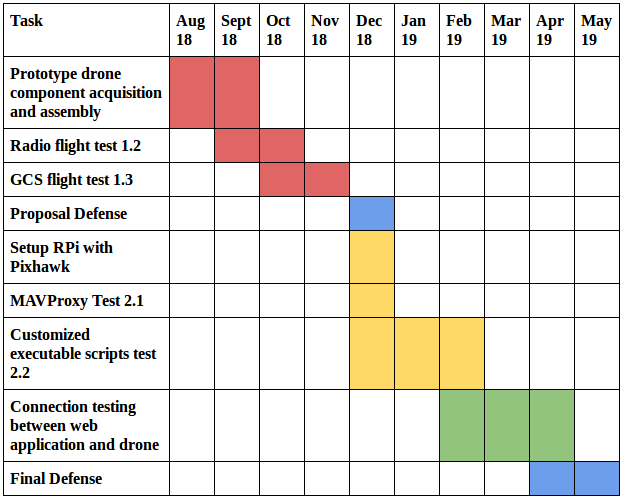
\includegraphics[width=\textwidth]{Ch4/workplan}
	\caption{Project Implementation and Work Plan}
	\label{fig:workplan}
\end{figure}
\FloatBarrier
